\section{RESULTADOS Y DISCUSIÓN}

La validación del esquema de control secundario distribuido se organiza en dos niveles complementarios, T1 y T2, cuyos alcances difieren de manera deliberada. El nivel T1 corresponde a un benchmark numérico multicriterio en el que nueve configuraciones de control se someten a la misma planta, a la misma perturbación y a los mismos ocho criterios de aceptación, de modo que las diferencias observadas puedan atribuirse al algoritmo y no al modelo. El nivel T2 corresponde al banco físico HIL de seis nodos Raspberry Pi 5, donde el esquema propuesto se ejecuta sobre una red eléctrica de ocho barras con su capa de comunicación real, su cadencia determinista y sus retardos de entrega efectivos. Ninguno de los dos niveles, considerado por separado, sostiene las conclusiones de este trabajo; la combinación de ambos sí lo hace, y esa es la razón por la cual se presentan en un mismo capítulo.

Un aspecto que conviene declarar desde el inicio es el estatuto de las cifras. Todos los valores numéricos reportados en este capítulo provienen de artefactos certificados mediante huella SHA-256 y no de transcripción manual: el benchmark deja un archivo de métricas con su manifiesto, y el banco HIL deja una telemetría con su propio resumen criptográfico. Cada tabla de este capítulo puede rastrearse hasta el archivo que la originó, de manera que la discusión se apoya en evidencia verificable y no en la memoria del experimentador. Esta trazabilidad es también la razón por la cual las cifras se reproducen con la precisión con que fueron emitidas, sin redondeos ni interpolaciones que faciliten la lectura a costa de la fidelidad.

\subsection{Alcance y organización de la validación}

El nivel T1 mide el desempeño del algoritmo de control en condiciones controladas y repetibles. La planta empleada es algebraico-cinemática de tipo droop, conforme a la decisión de diseño D-13, es decir, un modelo incremental de estado estacionario que reproduce el acoplamiento potencia-frecuencia y potencia-tensión sin resolver la dinámica electromagnética de los convertidores. La simplificación es intencional: permite ejecutar nueve configuraciones bajo exactamente la misma planta, la misma semilla y la misma secuencia de eventos, condición indispensable para que la comparación sea atribuible al algoritmo. En este nivel se evalúan la velocidad de restitución, la calidad del reparto proporcional de potencia activa y reactiva, los errores residuales de tensión y frecuencia, el margen de estabilidad numérica del esquema discreto y el retardo crítico admisible.

El nivel T2 mide algo distinto. Sobre el clúster de hardware de borde se verifica la cadencia real de $2\text{ Hz}$ sostenida durante $300\text{ s}$, la entrega de estados por ZeroMQ entre agentes, la resolución del flujo de potencia sobre la red de ocho barras, la respuesta ante perturbaciones de demanda inyectadas en nodos físicos y el comportamiento de los recursos frente a sus límites de capacidad. Su limitación es simétrica a la del nivel T1: en el banco sólo se ejecuta el esquema propuesto, de modo que no habilita comparaciones algorítmicas ni afirmaciones de superioridad.

La separación de niveles responde a una razón epistemológica antes que logística. Un benchmark numérico no puede exhibir retardos de entrega, ni saturación de actuadores, ni acoplamiento electromagnético con una red; un banco físico no puede, en un plazo razonable, ejecutar nueve configuraciones bajo condiciones idénticas, con semilla fija y repetibilidad bit a bit. Cada nivel responde, por tanto, una pregunta distinta: T1 pregunta cuál algoritmo se comporta mejor bajo criterios idénticos; T2 pregunta si el algoritmo propuesto sigue funcionando cuando se le enfrenta a la física, al reloj y a la red.

Los dos niveles tampoco son ejercicios independientes: cada uno responde a actividades del diseño metodológico y conviene dejarlo explícito para que el alcance del capítulo se lea contra el compromiso que lo originó. El benchmark numérico aplica la ley deducida en la actividad 1.3 sobre la planta cuyos modelos provienen de las actividades 1.1 y 1.2, la somete a las perturbaciones de la actividad 4.1 y la evalúa con las métricas de la 4.3. El banco HIL corresponde al despliegue de las actividades 3.1 y 3.2 bajo esa misma perturbación física. La familia de fallas de comunicación es la evidencia directa de la actividad 3.3 —el proxy de contingencias— y de la 4.2 —la inyección de latencia, pérdida de paquetes y desconexión de enlaces—. La familia de excedente, cuando se ejecute, completará la actividad 4.1 en el régimen excedentario.


Un tercer elemento completa la organización: el experimento nodal de retenedores. Su ubicación dentro del nivel T1 obedece a que comparte con el benchmark el carácter numérico y la repetibilidad, pero su alcance es distinto, pues se ejecuta sobre un único nodo y no sobre una red. Por esa razón se reporta al final del nivel T1 y se declara explícitamente como ensayo independiente, de manera que no se le confunda con una prueba del acoplamiento multitasa.

El capítulo se ordena como sigue. En primer término se presenta el nivel T1: el protocolo y los criterios de aceptación, el desempeño en tiempo de asentamiento (Tabla~\ref{tab:res_t1_asentamiento}), la calidad de reparto y la estabilidad numérica (Tabla~\ref{tab:res_t1_calidad}), el contraste con las cotas teóricas, la validación del arnés mediante controles negativos y el experimento nodal de retenedores de frontera (Tabla~\ref{tab:res_retenedores}). En segundo término se presenta el nivel T2, organizado por las tres familias del marco de evaluación: la de déficit de capacidad, analizada en cinco fases temporales y en un perfil nodal de tensión; la de excedente de generación, declarada con su escenario y su criterio a la espera de corrida; y la de fallas de comunicación, reportada con su ensayo de resiliencia. Cierra el capítulo una discusión integrada y una síntesis (Tabla~\ref{tab:res_sintesis}). Las nueve figuras que acompañan a estas tablas se distribuyen a lo largo del capítulo y se referencian desde el texto que las discute.

\subsection{Nivel T1: benchmark canónico de control secundario}

El benchmark reúne cinco algoritmos de control secundario —estatismo puro, proporcional-integral centralizado, acción integral distribuida, consenso en tiempo finito y consenso en tiempo fijo— en sus variantes publicada y optimizada cuando ambas existen. Cada configuración se somete a la misma secuencia de escalones de carga y a la misma reconfiguración de referencias, y se evalúa contra ocho criterios de aceptación independientes. El resultado agregado se expresa como el número de criterios aprobados sobre ocho, lo que permite una lectura rápida sin renunciar al detalle por criterio.

\subsubsection{Protocolo, trazabilidad y criterios de aceptación}

La corrida canónica del benchmark corresponde al identificador \texttt{20261108T161211\_bench-v2\_seed42}, que reemplaza a \texttt{20261108T152458\_bench-v2\_seed42} —y esta, a \texttt{20261107T161041\_bench-v2\_seed42} y a \texttt{20261104T163357\_bench-v2\_seed42}— sin diferencias numéricas entre las cuatro, y se declara con el campo \texttt{canonical} en verdadero en su manifiesto. La huella del manifiesto es \texttt{115a6eb9...}, y es la que certifica la correspondencia entre las cifras reportadas y los artefactos que las produjeron. La semilla es única e idéntica para las nueve configuraciones, requisito sin el cual la comparación perdería su sentido.

La planta es algebraico-cinemática de tipo droop, según la decisión D-13, y opera con \texttt{boundary\_hold\_applied} en falso. Esta última condición tiene una consecuencia que se precisa más adelante: el retenedor de frontera no interviene en el benchmark, de manera que las cifras de este nivel no incorporan ningún efecto de extrapolación entre pasos de acoplamiento. Los criterios de aceptación son los siguientes:

\begin{itemize}
    \item \textbf{G1:} tiempo de asentamiento normativo $t_s \le 52.54\text{ s}$;
    \item \textbf{G2:} desviación pico a pico de frecuencia $\Delta f < 0.200\text{ Hz}$;
    \item \textbf{G3:} desviación del índice de reparto reactivo $\Delta \eta_Q < 0.020$;
    \item \textbf{G4:} desviación del índice de reparto activo $\Delta \eta_P < 0.020$;
    \item \textbf{G5:} error de tensión $e_V \le 0.005\text{ p.u.}$;
    \item \textbf{G6:} error de frecuencia $e_\omega \le 0.100\text{ Hz}$;
    \item \textbf{G7:} número de Courant-Friedrichs-Lewy espectral $\text{CFL} < 1.0$;
    \item \textbf{G8:} retardo crítico $\tau_{crit} \ge 50\text{ ms}$.
\end{itemize}

El criterio G1 se evalúa sobre la banda normativa de $0.100\text{ Hz}$ y su umbral coincide con la cota de Lyapunov del grafo de validación, lo que lo convierte en una prueba de doble filo: exige cumplir la norma y, simultáneamente, no exceder el peor caso analítico. Con el objeto de no perder información en el extremo rápido de la respuesta, se reportan además bandas relativas al escalón de $10$, $5$ y $2$ por ciento, que no sustituyen al criterio normativo sino que lo complementan. Los índices $\eta_Q$ y $\eta_P$ empleados en G3 y G4 son los definidos en \eqref{eq:share_index}; el número CFL de G7 se define como la mitad del producto adimensional de \eqref{eq:cfl_condition}, de manera que el umbral de divergencia $2.0$ de la condición espectral corresponde exactamente a un CFL unitario; y el retardo crítico de G8 se calcula según \eqref{eq:tau_crit}.

Los tiempos de asentamiento se obtuvieron conforme a la definición de banda de \eqref{eq:tset_band}: en las bandas relativas, el ancho se expresa como fracción del escalón aplicado, mientras que en la banda normativa se expresa como valor absoluto en hercios. La distinción no es menor, porque una misma respuesta puede cerrar la banda del $2$ por ciento en $46.00\text{ s}$ y registrar un valor distinto en la banda normativa sin que exista contradicción: se trata de dos criterios de parada diferentes aplicados a la misma trayectoria, y el reporte conjunto evita que la elección de uno de ellos determine el veredicto. Los errores residuales de tensión y frecuencia se calcularon con el índice \eqref{eq:rmse} sobre la ventana de régimen permanente de cada corrida.

\subsubsection{Desempeño en tiempo de asentamiento}

La Tabla~\ref{tab:res_t1_asentamiento} consolida los tiempos de asentamiento de las nueve configuraciones evaluadas. Se incluyen cuatro bandas: la normativa de $0.100\text{ Hz}$ y las relativas de $10$, $5$ y $2$ por ciento respecto del escalón aplicado. El símbolo $\infty$ indica que la señal no ingresó a la banda dentro de la ventana de observación.

\begin{table}[H]
    \centering
    \footnotesize
    \caption{Tiempos de asentamiento del benchmark T1 por controlador, modo y banda de evaluación. El veredicto corresponde al criterio G1 sobre la banda normativa de $0.100\text{ Hz}$.}
    \label{tab:res_t1_asentamiento}
    \begin{tabularx}{\textwidth}{|>{\raggedright\arraybackslash}p{3.1cm}|>{\centering\arraybackslash}p{1.7cm}|>{\centering\arraybackslash}X|>{\centering\arraybackslash}X|>{\centering\arraybackslash}X|>{\centering\arraybackslash}X|>{\centering\arraybackslash}p{2.4cm}|}
        \hline
        \textbf{Controlador} & \textbf{Modo} & \textbf{$t_s$ normativo (s)} & \textbf{$t_s$ 10\% (s)} & \textbf{$t_s$ 5\% (s)} & \textbf{$t_s$ 2\% (s)} & \textbf{Veredicto} \\
        \hline
        Droop puro & published & $\infty$ & $\infty$ & $\infty$ & $\infty$ & REPROBADO \\
        \hline
        Droop puro & optimized & $\infty$ & $\infty$ & $\infty$ & $\infty$ & REPROBADO \\
        \hline
        PI centralizado & published & 8.50 & 11.00 & 13.50 & 16.00 & APROBADO \\
        \hline
        PI centralizado & optimized & 7.00 & 11.50 & 12.50 & 17.50 & APROBADO \\
        \hline
        DAPI & published & 26.00 & 45.50 & 70.00 & $\infty$ & APROBADO \\
        \hline
        DAPI & optimized & 23.50 & 41.50 & 63.50 & $\infty$ & APROBADO \\
        \hline
        FTS & published & 21.50 & 33.00 & 45.50 & 62.50 & APROBADO \\
        \hline
        FTS & optimized & 15.50 & 23.00 & 31.00 & 41.50 & APROBADO \\
        \hline
        FxTS & published & 13.00 & 21.50 & 31.50 & 46.00 & APROBADO \\
        \hline
    \end{tabularx}
\end{table}

\begin{figure}[H]
    \centering
    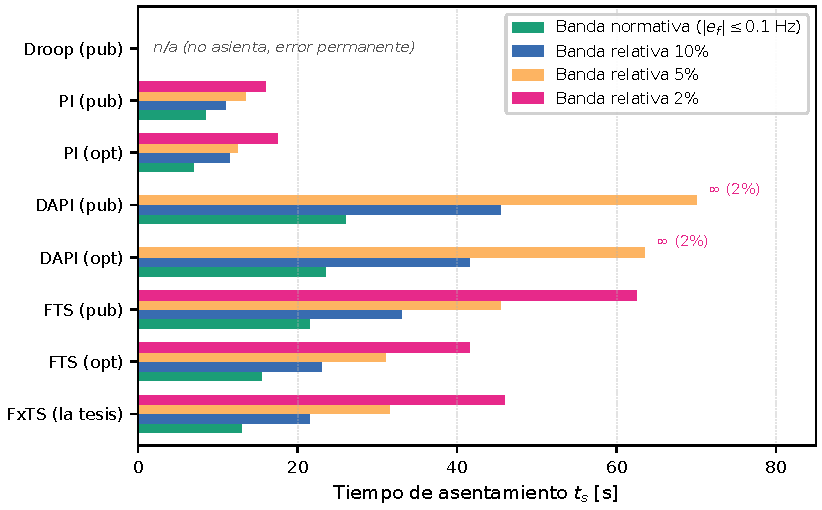
\includegraphics[width=0.95\textwidth]{Figuras/f5_1_tasas_asentamiento.pdf}
    \caption{Tiempos de asentamiento del nivel T1 por controlador y banda de evaluación: banda normativa de $0.100\text{ Hz}$ y bandas relativas de $10$, $5$ y $2$ por ciento. El estatismo puro no registra barra porque ninguna banda se cierra en la ventana de observación, y así se marca en el gráfico.}
    \label{fig:res_tasas_asentamiento}
\end{figure}

Tres lecturas se desprenden de la tabla. La primera es que el PI centralizado resultó el más rápido en la banda normativa, con $8.50\text{ s}$ en su variante publicada y $7.00\text{ s}$ en la optimizada, aunque su rapidez no viene acompañada de reparto de potencia, como se muestra en el apartado siguiente. La segunda es que el estatismo puro no asienta en ninguna de las cuatro bandas: sin lazo secundario, la desviación inducida por el estatismo es estacionaria por construcción y ninguna banda relativa llega a cerrarse dentro de la ventana. La tercera es la posición relativa del esquema propuesto: el FxTS asentó en $13.00\text{ s}$, esto es, $1.65$ veces más rápido que el FTS publicado ($21.50\text{ s}$) y $2$ veces más rápido que el DAPI publicado ($26.00\text{ s}$), sosteniendo además la banda del $2$ por ciento en $46.00\text{ s}$, donde el DAPI no la alcanza. La Figura~\ref{fig:res_tasas_asentamiento} ordena esas mismas mediciones por banda, de modo que se aprecia cuánto castiga cada exigencia adicional a cada controlador y en qué punto la comparación deja de ser posible porque ninguna banda llega a cerrarse.

Conviene subrayar el comportamiento del DAPI en la banda estrecha. Aunque aprueba el criterio normativo con $26.00\text{ s}$, su tiempo de asentamiento al $2$ por ciento es infinito en ambas variantes, lo que revela una cola de convergencia que la banda normativa no captura. El FTS y el FxTS, en cambio, cierran las cuatro bandas, y lo hacen en el orden esperado por la teoría: el esquema de tiempo fijo impone un plazo independiente del estado inicial, mientras que el de tiempo finito depende de la distancia inicial al equilibrio.

La comparación entre variantes publicada y optimizada aporta un dato adicional sobre la robustez de la sintonización. En el PI, la optimización mejoró la banda normativa de $8.50$ a $7.00\text{ s}$ pero degradó la banda del $2$ por ciento de $16.00$ a $17.50\text{ s}$, es decir, ganó velocidad inicial a costa de una cola más larga. En el DAPI y en el FTS el efecto fue uniforme, con mejoras en las cuatro bandas, mientras que el FxTS se reporta únicamente en su variante publicada porque el ajuste fino de sus exponentes no forma parte del alcance de esta validación. El estatismo, por su parte, no distingue entre variantes: ambas arrojan el mismo conjunto de valores, lo que confirma que su limitación no proviene de la sintonización sino de la ausencia de un lazo secundario.

\subsubsection{Calidad de reparto y estabilidad numérica}

La Tabla~\ref{tab:res_t1_calidad} reúne los seis indicadores restantes y el número de criterios aprobados por configuración. Las columnas $\Delta \eta_Q$ y $\Delta \eta_P$ cuantifican la dispersión del índice de utilización entre agentes; $e_V$ y $e_\omega$ son los errores residuales de tensión y frecuencia; CFL es el número espectral definido sobre \eqref{eq:cfl_condition}, y $\tau_{crit}$ el retardo crítico de \eqref{eq:tau_crit}. La abreviatura N/A señala que el indicador no es calculable por no existir capa de consenso distribuido o por no admitir el esquema un retardo finito de referencia.

\begin{table}[H]
    \centering
    \scriptsize
    \setlength{\tabcolsep}{3pt}
    \caption{Calidad de reparto, errores residuales, estabilidad numérica y criterios aprobados en el benchmark T1. CFL corresponde a la mitad del producto de \eqref{eq:cfl_condition}.}
    \label{tab:res_t1_calidad}
    \begin{tabularx}{\textwidth}{|>{\raggedright\arraybackslash}p{2.5cm}|>{\centering\arraybackslash}p{1.35cm}|>{\centering\arraybackslash}X|>{\centering\arraybackslash}X|>{\centering\arraybackslash}X|>{\centering\arraybackslash}X|>{\centering\arraybackslash}X|>{\centering\arraybackslash}X|>{\centering\arraybackslash}X|>{\centering\arraybackslash}p{1.55cm}|}
        \hline
        \textbf{Controlador} & \textbf{Modo} & \textbf{$\Delta f$ p-p (Hz)} & \textbf{$\Delta \eta_Q$} & \textbf{$\Delta \eta_P$} & \textbf{$e_V$ (p.u.)} & \textbf{$e_\omega$ (Hz)} & \textbf{CFL} & \textbf{$\tau_{crit}$ (ms)} & \textbf{Gates} \\
        \hline
        Droop puro & published & 0.0000 & 0.0800 & 0.1867 & 0.2000 & 0.4667 & 0.00 & N/A & 1 de 8 \\
        \hline
        Droop puro & optimized & 0.0000 & 0.0800 & 0.1867 & 0.2000 & 0.4667 & 0.00 & N/A & 1 de 8 \\
        \hline
        PI centralizado & published & 0.0000 & 0.0800 & 0.1867 & 0.0001 & 0.0000 & 0.25 & N/A & 5 de 8 (G8 no aplica) \\
        \hline
        PI centralizado & optimized & 0.0000 & 0.0800 & 0.1867 & 0.0000 & 0.0000 & 0.25 & N/A & 5 de 8 (G8 no aplica) \\
        \hline
        DAPI & published & 0.0120 & 0.0000 & 0.0000 & 0.0088 & 0.0236 & 0.16 & 2579.8 & 7 de 8 \\
        \hline
        DAPI & optimized & 0.0107 & 0.0000 & 0.0000 & 0.0067 & 0.0198 & 0.18 & 2299.8 & 7 de 8 \\
        \hline
        FTS & published & 0.0075 & 0.0000 & 0.0000 & 0.0000 & 0.0063 & 0.81 & 118.9 & 8 de 8 \\
        \hline
        FTS & optimized & 0.0017 & 0.0047 & 0.0047 & 0.0017 & 0.0009 & 1.60 & $-187.0$ & 6 de 8 \\
        \hline
        FxTS & published & 0.0029 & 0.0000 & 0.0000 & 0.0000 & 0.0018 & 0.84 & 96.3 & 8 de 8 \\
        \hline
    \end{tabularx}
\end{table}

\begin{figure}[H]
    \centering
    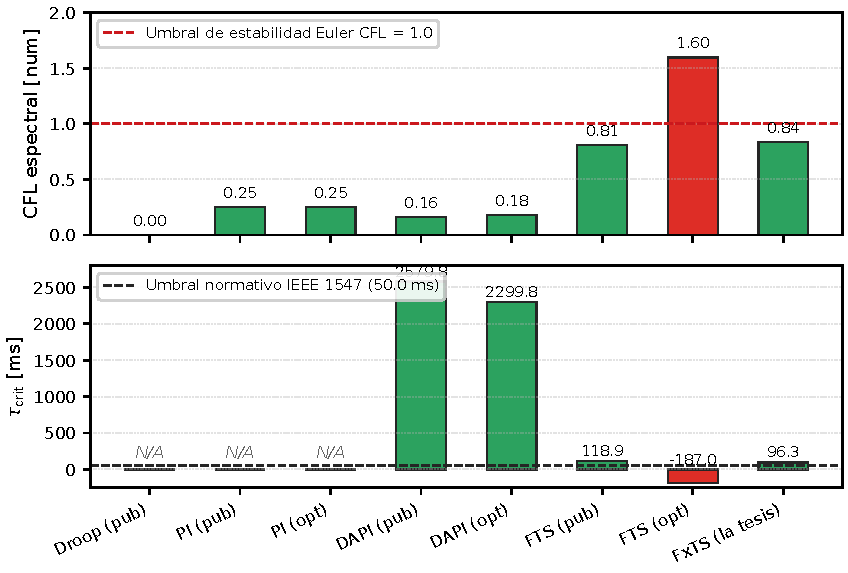
\includegraphics[width=0.95\textwidth]{Figuras/f5_6_estabilidad_numerica.pdf}
    \caption{Estabilidad numérica del benchmark T1. El panel superior compara el número CFL de cada configuración con el umbral unitario del criterio G7; el inferior, el retardo crítico con el umbral normativo de $50\text{ ms}$ del criterio G8. Las configuraciones sin capa de consenso distribuido no admiten retardo crítico y se marcan N/A, no cero.}
    \label{fig:res_estabilidad}
\end{figure}

El estatismo y el PI centralizado fallan G3 y G4 con idénticos valores de dispersión, $0.0800$ y $0.1867$ respectivamente. La causa no es un mal sintonizado sino estructural: ninguno de los dos esquemas incorpora acoplamiento entre vecinos, de modo que cada unidad se regula contra su propia referencia y la utilización relativa queda determinada por las impedancias y por los coeficientes de caída, no por un acuerdo explícito. El PI, en cambio, sí aprueba G1, G2, G5, G6 y G7, y su octavo criterio no aplica porque no existe capa de consenso distribuido sobre la cual definir un retardo crítico; de ahí el registro de $5$ de $8$ con la anotación correspondiente.

El DAPI invierte el patrón: reparte de forma ideal, con $\Delta \eta_Q$ y $\Delta \eta_P$ nulos en ambas variantes, y mantiene la desviación de frecuencia pico a pico en $0.0120\text{ Hz}$ y $0.0107\text{ Hz}$, valores reducidos frente al umbral de $0.200\text{ Hz}$. Sin embargo, falla G5 con $0.0088\text{ p.u.}$ en la variante publicada y $0.0067\text{ p.u.}$ en la optimizada, es decir, con un error de tensión entre una y dos veces el umbral de $0.005\text{ p.u.}$. El resultado es coherente con la naturaleza del lazo: la acción integral distribuida restituye la frecuencia y el reparto, pero no dispone de una señal de tensión con la misma autoridad, de manera que la regulación de magnitud queda rezagada.

El caso del FTS optimizado merece atención porque muestra que la optimización de ganancias puede comprar velocidad a costa de estabilidad numérica. Al elevar la ganancia, el esquema reduce el tiempo de asentamiento normativo de $21.50\text{ s}$ a $15.50\text{ s}$, pero viola G7 con un CFL de $1.60$ y G8 con un retardo crítico negativo de $-187.0\text{ ms}$. Un $\tau_{crit}$ negativo no significa que el lazo tolere retardos pequeños: significa que el esquema discreto ya es inestable en ausencia de retardo, y que ninguna reducción del mismo puede restituir la estabilidad. Sólo el FTS publicado y el FxTS publicado aprueban los ocho criterios, y lo hacen con márgenes distintos: el FxTS con CFL de $0.84$ y $\tau_{crit}$ de $96.3\text{ ms}$, el FTS con CFL de $0.81$ y $\tau_{crit}$ de $118.9\text{ ms}$. La Figura~\ref{fig:res_estabilidad} sitúa ambos indicadores frente a sus umbrales: en el panel superior el CFL de cada configuración contra la unidad, y en el inferior el retardo crítico frente a su umbral normativo, con las configuraciones que no admiten retardo marcadas como no aplicables en lugar de cero.

\subsubsection{Contraste con las cotas teóricas}

El primer contraste es el de la cota de Lyapunov. Para el grafo lineal de tres agentes, con conectividad algebraica $\lambda_2 = 1.0$, la cota de asentamiento derivada en el capítulo teórico es $T_f \le 52.54\text{ s}$, valor que coincide con el umbral del criterio G1. El FxTS asentó en $13.00\text{ s}$, esto es, un factor $4.04$ por debajo de la cota. La lectura correcta de ese factor no es que el algoritmo sea cuatro veces mejor de lo que promete, sino que la cota es un peor caso global construido para condiciones iniciales arbitrariamente alejadas del equilibrio, mientras que la operación de una microrred mantiene las desviaciones acotadas; la cota se cumple con holgura porque el régimen real es local.

El segundo contraste es el de la condición espectral. Con paso de discretización $\Delta t = 0.5\text{ s}$, autovalor máximo $\lambda_{\max}(\mathcal{H}) = 3.247$ y ganancia efectiva $g_{\text{ef}} = 1.033$ en el interior de la capa límite, el producto de \eqref{eq:cfl_condition} resulta $1.677$, inferior al límite de $2.0$ con un margen de $16.2$ por ciento, equivalente a un factor de $1.19$ entre el umbral y el valor efectivo. El CFL reportado en la Tabla~\ref{tab:res_t1_calidad} es precisamente ese producto dividido por dos, de donde resulta $0.84$; la normalización permite comparar el margen contra la unidad y explica por qué el umbral de G7 se fija allí y no en $2.0$.

El tercer contraste es el del retardo. La cota analítica de \eqref{eq:tau_crit} arroja $96.3\text{ ms}$ para la topología de validación, frente al umbral normativo de $50\text{ ms}$ adoptado en G8, lo que representa un factor de $1.93$ de holgura. El resultado es relevante porque el retardo crítico no se estimó por búsqueda empírica sino que se despejó de la misma condición de contracción que gobierna el CFL; ambos indicadores son, por tanto, dos vistas del mismo margen, y su consistencia mutua constituye una verificación cruzada del modelo de estabilidad.

\subsubsection{Validación del arnés mediante controles negativos}

Un benchmark que sólo reporta aprobados no demuestra que sepa reprobar. Por esa razón el arnés se sometió a cuatro controles negativos, cuyo propósito es verificar que el instrumento detecta las fallas que debe detectar y que el aprobado del esquema propuesto no es vacuo.

El control N1 anuló el consenso, dejando la ley de actualización sin término de vecinos. El resultado fue la ausencia de restitución: los errores residuales se mantuvieron en el valor inducido por el estatismo y ningún criterio de reparto se satisfizo. El control N2 sustituyó las ganancias por valores ajenos al diseño, $0.15$ y $0.85$, con los cuales el CFL igualó o superó la unidad y el esquema discreto perdió la contracción. El control N3 invirtió el signo del término restaurativo, lo que produjo divergencia y confirmó que la retroalimentación negativa es la que sostiene la convergencia. El control N4 empleó el DAPI como control positivo: al ser un esquema correctamente formulado, aprobó siete criterios y sólo quedó en reserva por G5, con un error de tensión de $0.0088\text{ p.u.}$.

El conjunto de los cuatro controles delimita el comportamiento del arnés: detecta la ausencia de acoplamiento, detecta el exceso de ganancia, detecta la inversión de signo y no penaliza indebidamente a un esquema ajeno bien formulado. El aprobado de ocho sobre ocho del FxTS se interpreta, por tanto, contra un instrumento que ya demostró saber fallar en las condiciones en que corresponde fallar.

\subsubsection{Experimento nodal de retenedores de frontera}

El benchmark no incorpora retenedores de frontera, pues opera con \texttt{boundary\_hold\_applied} en falso; el estudio de retenedores constituye, en consecuencia, un experimento nodal independiente y así se declara. El ensayo se ejecutó sobre el nodo solar de tipo Boost, con consigna de reactiva $Q_{\text{ref}} = 4000\text{ var}$, consigna activa $P_{\text{ref}} = 0\text{ W}$, irradiancia de $800\text{ W/m}^2$ y temperatura de $25$ grados. En $t = 40\text{ s}$ se impuso una caída de tensión a $0.8\text{ p.u.}$ con constante de $4.5\text{ s}$, y el registro se extendió durante $120\text{ s}$. Cada retenedor operó con paso de $0.5\text{ s}$ y se comparó contra una referencia calculada con paso de $0.05\text{ s}$, de manera que el error reportado mide el efecto de retener el estado de frontera durante un macro-paso completo.

\begin{table}[H]
    \centering
    \footnotesize
    \caption{Error de retención de la potencia del nodo solar Boost frente a la referencia de paso fino. El factor se calcula respecto del retenedor de orden cero.}
    \label{tab:res_retenedores}
    \begin{tabularx}{\textwidth}{|>{\raggedright\arraybackslash}p{3.6cm}|>{\centering\arraybackslash}X|>{\centering\arraybackslash}X|>{\centering\arraybackslash}X|}
        \hline
        \textbf{Retenedor} & \textbf{RMS (W)} & \textbf{Máximo (W)} & \textbf{Factor frente a ZOH} \\
        \hline
        ZOH & 3.85 & 26.65 & 1.00 \\
        \hline
        FROH $\lambda = 0.3$ & 7.45 & 110.31 & 1.93 \\
        \hline
        FROH $\lambda = 0.5$ & 10.80 & 166.09 & 2.80 \\
        \hline
        FROH $\lambda = 0.7$ & 14.33 & 221.87 & 3.72 \\
        \hline
        FROH $\lambda = 0.9$ & 17.93 & 277.65 & 4.65 \\
        \hline
        FOH ($\lambda = 1.0$) & 19.74 & 305.54 & 5.12 \\
        \hline
    \end{tabularx}
\end{table}

\begin{figure}[H]
    \centering
    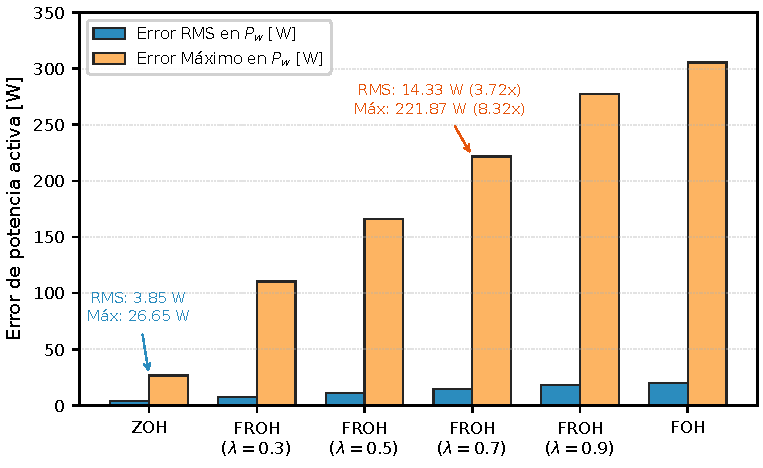
\includegraphics[width=0.95\textwidth]{Figuras/f5_7_retenedores.pdf}
    \caption{Error de retención de la potencia del nodo solar Boost para los seis esquemas evaluados, en RMS y en máximo frente a la referencia de paso fino. Las cifras anotadas coinciden con la Tabla~\ref{tab:res_retenedores}.}
    \label{fig:res_retenedores}
\end{figure}

El resultado contradice la expectativa habitual de que un retenedor de orden superior reduce el error de acoplamiento. El ZOH fue el más preciso de la serie, con un RMS de $3.85\text{ W}$ y un máximo de $26.65\text{ W}$, mientras que todas las variantes de extrapolación lo superaron, y el FOH elevó su error máximo a $305.54\text{ W}$ y su error RMS a $19.74\text{ W}$, esto es, un factor de $5.12$ sobre el RMS del ZOH. La explicación es mecánica: el retenedor implementado en el código extrapola con diferencia retrospectiva, es decir, opera como un predictor de primer orden construido sobre el último par de muestras. En una dinámica convexa como la caída de tensión con constante de $4.5\text{ s}$, la extrapolación lineal sobreestima sistemáticamente la señal, y el sesgo crece con el horizonte de predicción, que es precisamente lo que el parámetro $\lambda$ escala. La Figura~\ref{fig:res_retenedores} presenta la serie completa con el error RMS y el máximo en paralelo, de modo que se observa que el deterioro acompaña al parámetro de extrapolación y no se concentra en un caso aislado.

Debe precisarse que este retenedor no es el de Ishitobi, pese a la similitud de la nomenclatura. El esquema aquí evaluado no resuelve la condición de empalme de la trayectoria entre muestras, sino que prolonga la secante; su comportamiento es el de un predictor y no el de un reconstructor de orden fraccionario. El cociente máximo entre la señal retenida y la de referencia llegó a $8.33$ en el peor caso, lo que confirma que la extrapolación agresiva no es una mejora incremental sino una fuente de error dominante. La consecuencia práctica para la arquitectura de co-simulación es que el ZOH, pese a su simplicidad, constituye la opción conservadora y verificable, y que cualquier retenedor alternativo debería someterse a este mismo ensayo antes de adoptarse.

\subsection{Nivel T2: validación ciber-física en clúster HIL}

El nivel T2 traslada el esquema propuesto al hardware. El ensayo se ejecutó sobre el clúster de seis Raspberry Pi 5 y el PC Central, con la red de ocho barras, los recursos distribuidos en sus contenedores y la capa de comunicación ZeroMQ operando en modo lock-step. A diferencia del benchmark, aquí no hay variantes ni semillas: el ensayo de déficit es una sola ejecución de $300\text{ s}$ que se analiza por ventanas temporales, cada una asociada a un régimen operativo distinto. Ese ensayo cubre la primera de las tres familias del marco de evaluación, la de déficit de capacidad. La segunda, la de excedente de generación, cuenta con su escenario emitido e instalado pero no con corrida ejecutada, de modo que se declara con su criterio y sin cifras. La tercera, la de fallas de comunicación, se reporta con el ensayo de resiliencia que se describe en su apartado.

\subsubsection{Plataforma y contrato de muestreo}

El clúster se compone de seis Raspberry Pi 5 con direcciones \texttt{10.0.0.151} a \texttt{10.0.0.155} y \texttt{10.0.0.160}, coordinadas por el PC Central en \texttt{10.0.0.156} sobre una red Ethernet dedicada. La red eléctrica modelada es radial de baja tensión, con tensión nominal de $400\text{ V}$, ocho barras, siete ramas y potencia base de $10\text{ kVA}$. El contrato de muestreo establece $600$ pasos a $2\text{ Hz}$ con paso de $0.5\text{ s}$, lo que cubre $300\text{ s}$ de operación; la telemetría resultante consta de $600$ filas por $27$ columnas, con huella SHA-256 \texttt{bd71ba4a...}.

El paso correspondiente a $t = 0.0$ es un arranque plano previo al primer pulso del reloj ZeroMQ y, por esa razón, no se reporta: incluirlo introduciría en las estadísticas un estado que no pertenece a la operación del lazo cerrado. El ensayo se ejecutó sobre el escenario ESC-HIL-001\_rampa\_sombreado\_demanda, del que existe una versión consolidada —ESC-HIL-003\_consolidado\_rev5, la vigente en el banco— numéricamente equivalente: delta máximo nulo en las dieciocho series de entrada a lo largo de las $601$ muestras. Las series de irradiancia y de demanda que acompañan este capítulo provienen de los archivos consolidados de esa versión, de modo que las Figuras~\ref{fig:res_poa} y~\ref{fig:res_demanda} describen exactamente las entradas del ensayo. La ejecución se realizó con el lazo de potencia activa reconectado y con el anti-windup de $\pm 75\ \text{rad}$ de \eqref{eq:rest_local} en el integrador de frecuencia, de modo que la autoridad del agente quedó acotada durante los transitorios y no acumuló error mientras el actuador estaba saturado.

El contrato de muestreo merece una precisión adicional, porque de él depende la comparabilidad de las fases. Los $600$ pasos se ejecutaron en modo lock-step: el PC Central no avanzó al macro-paso siguiente hasta haber recibido las potencias de los seis nodos o hasta agotar el tiempo de espera configurado. Esa disciplina es la que permite afirmar que cada fila de la telemetría corresponde a un instante de simulación y no a un instante de llegada de mensajes, y es también la que sostiene la cadencia de $2\text{ Hz}$ como propiedad verificada y no como promedio. Las $27$ columnas registran, por nodo y por paso, las potencias activa y reactiva inyectadas, la magnitud y el ángulo de tensión de acoplamiento, la frecuencia local, los estados de consenso y los índices de utilización, de manera que cada afirmación de este apartado puede recalcularse a partir del archivo y no requiere del código que lo generó. Las Figuras~\ref{fig:res_poa} y~\ref{fig:res_demanda} recogen las series exógenas que gobiernan el ensayo, de modo que las respuestas de las fases siguientes puedan contrastarse contra la perturbación que las origina.

\begin{figure}[H]
    \centering
    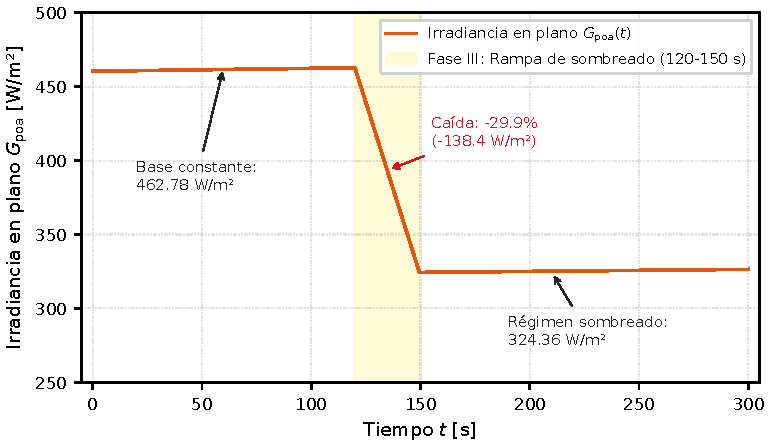
\includegraphics[width=0.95\textwidth]{Figuras/f5_8_poa.pdf}
    \caption{Irradiancia en el plano del arreglo durante los $300\text{ s}$ del ensayo, con la ventana de sombreado de la fase III delimitada. La serie se mantiene en $462.78\text{ W/m}^2$ hasta $t = 120\text{ s}$, desciende hasta $324.36\text{ W/m}^2$ en $t = 150\text{ s}$ y permanece constante el resto del ensayo; la caída es de $138.4\text{ W/m}^2$, el $29.9$ por ciento.}
    \label{fig:res_poa}
\end{figure}
\begin{figure}[H]
    \centering
    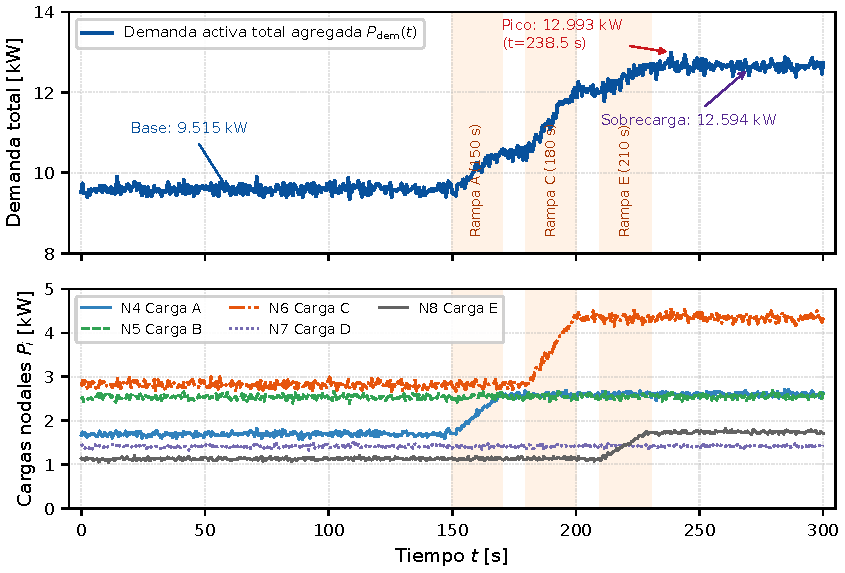
\includegraphics[width=0.95\textwidth]{Figuras/f5_9_demanda.pdf}
    \caption{Demanda del ensayo HIL. El panel superior muestra la demanda agregada, con la base de $9.515\text{ kW}$, el pico de $12.993\text{ kW}$ y el régimen de sobrecarga de $12.594\text{ kW}$, y señala el arranque de las tres rampas en $150$, $180$ y $210\text{ s}$; el panel inferior desglosa las cinco cargas nodales.}
    \label{fig:res_demanda}
\end{figure}

\subsubsection{Familia 1: déficit de capacidad}

La primera familia del marco reúne el ensayo en el que la demanda llega a exceder la capacidad firme del conjunto, de modo que la frecuencia no puede sostenerse sin la acción conjunta del estatismo primario y del lazo secundario. Su evidencia es una única ejecución sobre el clúster que se analiza en cinco ventanas temporales, cada una asociada a un régimen operativo distinto, y en un perfil de tensión nodal que se presenta al cierre de la familia.

\subsubsection{Fase I: acoplamiento y convergencia inicial}

La primera ventana abarca de $0.5$ a $25\text{ s}$ y corresponde al acoplamiento inicial entre el lazo físico y el lazo de consenso. La potencia neta intercambiada con la red osciló entre $-8.52$ y $+1.21\text{ kW}$, rango amplio que refleja la acomodación de los recursos desde el arranque plano hasta el punto de operación. La frecuencia registró su mínimo transitorio de $59.0556\text{ Hz}$ en $t = 9.0\text{ s}$.

El dato relevante de la fase es la convergencia del lazo reactivo. El consenso de reactiva convergió en el paso $21$, correspondiente a $t = 10.5\text{ s}$, con errores $e_{Q12}$ y $e_{Q23}$ iguales a $0.0000$. A partir de ese instante, el índice de utilización reactiva se mantuvo en $30.74$ por ciento en los tres inversores y así permaneció durante el resto del ensayo. La convergencia en $10.5\text{ s}$ debe contrastarse con la cota de $52.54\text{ s}$ del apartado anterior: el lazo físico converge dentro del plazo teórico y con un margen consistente con el factor observado en el benchmark. La Figura~\ref{fig:res_consenso_reactiva} registra ese cierre en sus dos paneles: la magnitud de los errores de consenso y los índices de utilización de los tres inversores, que dejan de separarse una vez alcanzada la convergencia.

El recorrido de la potencia neta en esta ventana, entre $-8.52$ y $+1.21\text{ kW}$, es propio del transitorio de acoplamiento y se atenúa una vez que el lazo secundario toma autoridad sobre las consignas. Su amplitud no indica una falla de reparto sino la acomodación de los convertidores desde el arranque plano, en el que ninguna unidad ha fijado aún su punto de operación. La excursión de $59.0556\text{ Hz}$ registrada en $t = 9.0\text{ s}$ es de amplitud comparable a la de la fase de sobrecarga y ocurre antes de que el consenso tome autoridad, lo que confirma que responde a la energización del conjunto y no a un déficit de capacidad. Las Figuras~\ref{fig:res_frecuencia_hil} y~\ref{fig:res_potencia_neta} amplían la mirada al registro completo: en la primera las cinco fases del banco quedan delimitadas, de modo que la excursión de esta ventana se compara con las posteriores; en la segunda las rampas de demanda se señalan sobre la traza de potencia neta.

\begin{figure}[H]
    \centering
    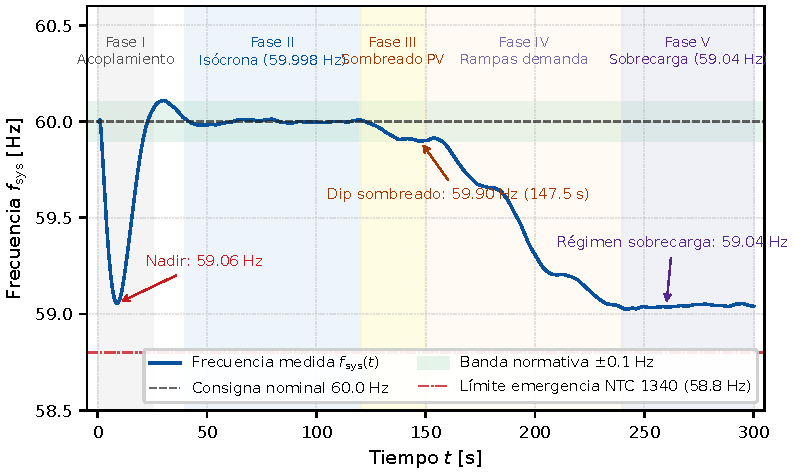
\includegraphics[width=0.95\textwidth]{Figuras/f5_2_frecuencia_hil.pdf}
    \caption{Frecuencia del sistema durante los $300\text{ s}$ del ensayo HIL, con las cinco fases del banco delimitadas por bandas sombreadas. Las guías horizontales señalan la ventana de la NTC 1340 y la banda fina de $0.1\text{ Hz}$; el eje vertical está restringido a la zona de interés y no cubre el rango completo de operación.}
    \label{fig:res_frecuencia_hil}
\end{figure}
\begin{figure}[H]
    \centering
    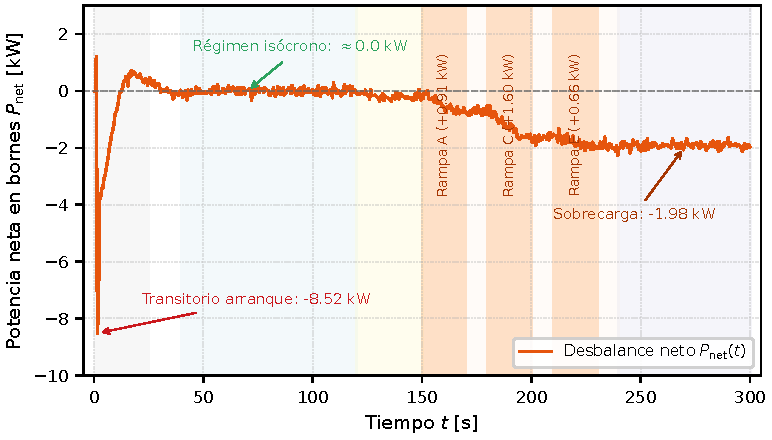
\includegraphics[width=0.95\textwidth]{Figuras/f5_3_potencia_neta.pdf}
    \caption{Potencia neta intercambiada con la red durante los $300\text{ s}$ del ensayo HIL. Las tres rampas de demanda se señalan sobre la traza y las anotaciones marcan el mínimo del transitorio de acoplamiento y el régimen de sobrecarga; el eje vertical es simétrico respecto de cero.}
    \label{fig:res_potencia_neta}
\end{figure}
\begin{figure}[H]
    \centering
    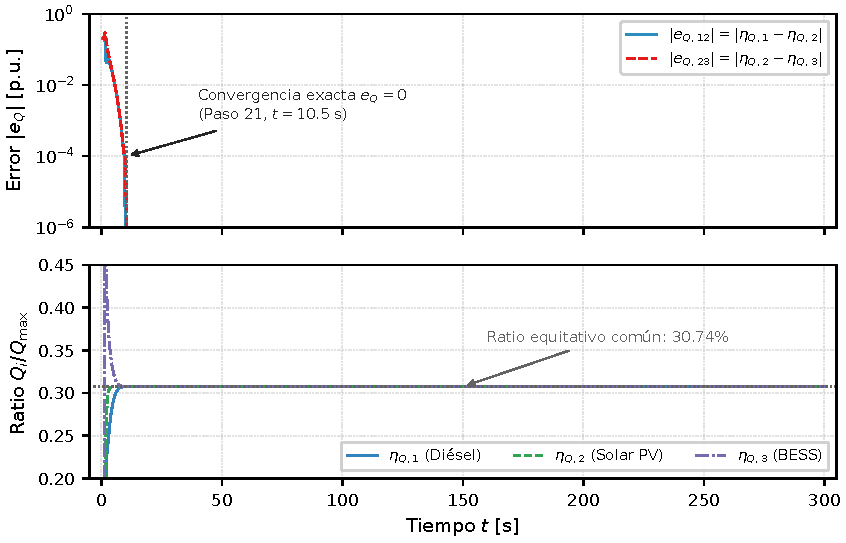
\includegraphics[width=0.95\textwidth]{Figuras/f5_5_consenso_reactiva.pdf}
    \caption{Consenso de potencia reactiva en el ensayo HIL, durante los $300\text{ s}$ del registro. El panel superior muestra la magnitud de los errores de consenso en escala logarítmica; el inferior, los índices de utilización reactiva de los tres inversores. La convergencia exacta de ambos errores se alcanza en el paso 21.}
    \label{fig:res_consenso_reactiva}
\end{figure}

\subsubsection{Fase II: régimen isócrono}

Entre $40$ y $120\text{ s}$ el sistema operó en régimen isócrono. La frecuencia se mantuvo en $59.9983 \pm 0.0082\text{ Hz}$, con un mínimo de $59.9815\text{ Hz}$ y un máximo de $60.0139\text{ Hz}$; la desviación media respecto de $60.0\text{ Hz}$ fue de $0.0017\text{ Hz}$. La potencia neta promedió $-0.0027\text{ kW}$, con un rango de $-0.32$ a $+0.29\text{ kW}$, y la demanda agregada promedió $9.5983\text{ kW}$, con valores entre $9.3417$ y $9.8969\text{ kW}$. La interpretación de esta ventana es directa: el lazo integral del generador diésel sostiene el punto isócrono, de modo que la frecuencia permanece próxima a la nominal sin que el consenso deba intervenir con autoridad adicional. La dispersión observada corresponde al ruido de cuantización del reloj y no a una oscilación de lazo, y la irradiancia se mantiene constante a lo largo de todo el intervalo, de modo que ninguna perturbación de recurso actúa todavía sobre el sistema.

\subsubsection{Fase III: sombreado fotovoltaico}

Entre $120$ y $150\text{ s}$ el escenario aplica la rampa de sombreado fotovoltaico definida en ESC-HIL-001, que no constituye una contingencia no modelada sino una perturbación declarada del guion de ensayo. Hasta $t = 120\text{ s}$ la irradiancia se mantiene en $462.78\text{ W/m}^2$; a partir de ese instante desciende de forma continua hasta $324.36\text{ W/m}^2$ en $t = 150\text{ s}$, esto es, una reducción de $138.42\text{ W/m}^2$ equivalente al $29.91$ por ciento en treinta segundos, y desde ahí permanece constante. La Figura~\ref{fig:res_poa} presenta esa rampa sobre el registro completo del ensayo. La demanda agregada no cambia en esta ventana: promedia $9.5875\text{ kW}$ y oscila entre $9.3935$ y $9.7886\text{ kW}$. La perturbación es, por tanto, de recurso y no de carga, condición que permite atribuirle el desplazamiento de frecuencia que se observa a continuación.

La consecuencia medida es un descenso de la frecuencia a $59.9394 \pm 0.0373\text{ Hz}$, con mínimo de $59.8979\text{ Hz}$ en $t = 147.5\text{ s}$, equivalente a una desviación de $0.1021\text{ Hz}$ respecto de la nominal. La potencia neta promedia $-0.1769\text{ kW}$ y alcanza su mínimo de $-0.37\text{ kW}$ en $t = 130.5\text{ s}$. La frecuencia cruza la banda de $0.100\text{ Hz}$ en $t = 146.5\text{ s}$, sin que se registre desconexión de carga ni actuación de protecciones. La correlación entre irradiancia y frecuencia en esta ventana es de $+0.954$, frente a $+0.313$ en la ventana isócrona, donde la irradiancia es constante; ese contraste sostiene la atribución causal.

La interpretación física concuerda con la magnitud del fenómeno. La caída de generación fotovoltaica es del orden de $0.23\text{ kW}$ y la absorbe el respaldo proporcional del diésel, cuyo aporte es $\kappa_{p,\omega} e_\omega \approx 95\text{ W}$ para la desviación media y $\approx 160\text{ W}$ en el mínimo, del mismo orden que el desbalance medido. El lazo integral no alcanza a cerrar el error antes de que comiencen las rampas de demanda de la fase siguiente, de manera que el sistema llega a esa fase con un desplazamiento cercano a $0.10\text{ Hz}$ que no le corresponde.

\subsubsection{Fase IV: perturbaciones de demanda}

Entre $150$ y $238.5\text{ s}$ se inyectaron tres rampas de demanda de $20\text{ s}$ de duración cada una: en el nodo N4 un incremento de $0.906\text{ kW}$ entre $150$ y $170\text{ s}$; en el nodo N6 un incremento de $1.596\text{ kW}$ entre $180$ y $200\text{ s}$; y en el nodo N8 un incremento de $0.657\text{ kW}$ entre $210$ y $230\text{ s}$. La Figura~\ref{fig:res_demanda} sitúa las tres rampas sobre la demanda agregada y desglosa las cinco cargas nodales. Aquí comienza la componente de demanda de la perturbación, sobre un sistema que ya venía desplazado en cerca de $0.10\text{ Hz}$ por el sombreado de la fase anterior. Las tres rampas se suceden sin solaparse entre sí, lo que permitió observar la respuesta del lazo integral a medida que la carga crecía de forma escalonada.

La demanda agregada pasó de $9.515\text{ kW}$ a $12.594\text{ kW}$ en $t = 240\text{ s}$, con un pico de $12.993\text{ kW}$ en $t = 238.5\text{ s}$ asociado al último escalón de la rampa. El incremento total, del orden de $3.5\text{ kW}$ sobre una base de $9.515\text{ kW}$, sometió a los recursos a una exigencia superior a su capacidad firme, situación que se resolvió en la fase siguiente y que constituye el fenómeno central de la validación en hardware.

La respuesta durante las rampas conservó la forma prevista: la frecuencia descendió de manera gradual mientras la demanda crecía, el reparto activo se mantuvo equitativo entre los agentes y la tensión nodal no se separó de la referencia. La suavidad de la excursión se explica por la duración de cada rampa, de $20\text{ s}$, muy superior a la constante de tiempo del lazo secundario, de modo que el consenso dispuso de tiempo para redistribuir la carga sin que el sistema operara fuera de su punto de equilibrio cuasiestático. Al finalizar la tercera rampa, sin embargo, la demanda superó el techo de capacidad y el régimen cambió de naturaleza.

\subsubsection{Fase V: sobrecarga y transición al estatismo primario}

Entre $240$ y $300\text{ s}$ el sistema operó en sobrecarga. La frecuencia se estabilizó en $59.0414 \pm 0.0076\text{ Hz}$, con un mínimo de $59.0247\text{ Hz}$ en $t = 242.0\text{ s}$, correspondiente al paso $484$. La potencia neta fue de $-1.980\text{ kW}$ en $t = 240\text{ s}$ y de $-1.970\text{ kW}$ en $t = 300\text{ s}$, es decir, prácticamente constante a lo largo de la ventana.

La deducción de esta condición operativa se desarrolla a continuación. La potencia generada real resultó de descontar a la demanda el intercambio neto con la red:

\begin{equation}
P_{\text{gen}} = P_{\text{dem}} - P_{\text{net}} = 12.594 - 1.980 = 10.614\ \text{kW}
\end{equation}

Esa potencia se repartió entre los tres recursos del banco. El nodo solar aportó $0.535\text{ kW}$ con una irradiancia cercana a $325.6\text{ W/m}^2$, el BESS entregó $1.500\text{ kW}$, valor que corresponde a su límite continuo, y el diésel asumió el resto con $8.579\text{ kW}$ eléctricos:

\begin{equation}
P_{\text{eje}} = \frac{8.579}{0.95} = 9.03\ \text{kW}
\end{equation}

donde $0.95$ es el rendimiento adoptado para el conjunto generador. La capacidad firme a $60.0\text{ Hz}$ se obtiene sumando la capacidad del diésel, la del BESS y el aporte solar disponible:

\begin{equation}
P_{\text{firme}} = 9.500 + 1.500 + 0.535 = 11.535\ \text{kW}
\end{equation}

de modo que el déficit de capacidad frente a la demanda de la fase resulta:

\begin{equation}
\Delta P = P_{\text{dem}} - P_{\text{firme}} = 12.594 - 11.535 = -1.059\ \text{kW}
\end{equation}

El déficit explica la caída de frecuencia sin necesidad de invocar una falla del algoritmo. Para verificarlo, se contrastó el valor medido con la predicción de la ecuación de oscilación \eqref{eq:swing}, evaluada con potencia base de $10\text{ kVA}$ y coeficiente de amortiguamiento de $12$:

\begin{equation}\label{eq:res_swing_pred}
f_{\text{pred}} = 60.0 + \frac{1}{12}\cdot\frac{-1.980}{10}\cdot 60.0 = 59.010\ \text{Hz}
\end{equation}

La predicción de $59.010\text{ Hz}$ corresponde al valor de régimen permanente del modelo rígido. La frecuencia medida, $59.0414\text{ Hz}$, se ubica por encima de esa predicción porque la señal atraviesa el filtro pasa-bajos de constante $2.0\text{ s}$ antes de ser registrada, lo que suaviza el escalón y reduce la excursión. La convergencia entre ambos valores, del orden de tres centésimas de hercio, confirma que la ecuación de oscilación describe adecuadamente el fenómeno y que la diferencia es atribuible al filtrado de medición y no a una dinámica no modelada.

El respaldo proporcional del diésel se verificó sobre el estatismo de \eqref{eq:droop_w}. Con una desviación de frecuencia de $6.023\text{ rad/s}$ respecto de la referencia y la ganancia $\kappa_{p,\omega} = 250.0\ \text{W/(rad/s)}$ declarada en \eqref{eq:rest_local}, la potencia adicional entregada por el gobernador resulta:

\begin{equation}
P_{\text{res}} = 250.0 \times 6.023 = 1505.7\ \text{W}
\end{equation}

Este respaldo, sumado al punto de operación previo del generador, es el que sostiene la frecuencia en $59.04\text{ Hz}$ en lugar de permitir una caída mayor. La transición hacia el estatismo primario fue monótona: no se observaron ciclos límite, ni oscilaciones sostenidas, ni actuación del relé de subfrecuencia.

\subsubsection{Perfil de tensión nodal}

La tensión en las ocho barras se mantuvo entre $0.99965$ y $1.00462\text{ p.u.}$, es decir, entre $399.86$ y $401.85\text{ V}$ sobre la base de $400\text{ V}$. El rango completo de variación nodal fue, por tanto, inferior a medio punto porcentual, muy por debajo de la tolerancia de $\pm 5$ por ciento que admiten IEEE 1547 y la norma NTC 1340. El resultado es consistente con la operación del lazo de restitución de tensión: el error $e_V$ reportado en el benchmark fue nulo, y en el banco la tensión no llegó a separarse de la referencia en ninguna barra ni durante las rampas de demanda. La Figura~\ref{fig:res_tensiones} recoge la envolvente de las ocho barras a lo largo del ensayo con el eje vertical ampliado a la zona de interés, de modo que se aprecia la forma de la variación aunque el margen frente a la tolerancia regulatoria no resulte visible a esa escala.

\begin{figure}[H]
    \centering
    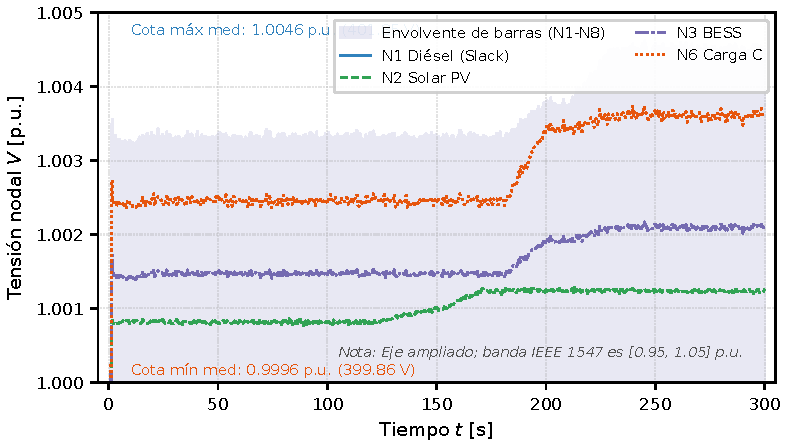
\includegraphics[width=0.95\textwidth]{Figuras/f5_4_tensiones_nodales.pdf}
    \caption{Envolvente de tensión de las ocho barras durante el ensayo HIL. El eje vertical está ampliado a la zona de interés, de $1.000$ a $1.005\text{ p.u.}$, y por tanto no representa la tolerancia completa de $\pm 5$ por ciento de IEEE 1547 y NTC 1340.}
    \label{fig:res_tensiones}
\end{figure}

\subsubsection{Familia 2: excedente de generación}

La segunda familia del marco de evaluación invierte el signo del balance. En ella la demanda nunca supera la generación disponible, de modo que la frecuencia no está en riesgo por insuficiencia, pero la generación sí puede superar la demanda y el excedente debe absorberse o recortarse. El escenario correspondiente está emitido e instalado, pendiente de ensayo, y exige una ventana declarada con irradiancia elevada y demanda plana o descendente: la perturbación inversa a la del ensayo anterior, donde el sombreado redujo la generación manteniendo la carga constante.

Lo que se medirá en esa ventana es, primero, la frecuencia sostenida dentro de $\pm 0.05\ \text{Hz}$ de la nominal; segundo, el reparto equitativo del exceso entre la carga de la batería y el recorte de la fuente fotovoltaica, con un índice de utilización propio y un error de consenso de la misma cota que el de la reactiva; y tercero, la ausencia de saturación de la absorción salvo en el límite declarado del BESS. Ambas capacidades están implementadas en la plataforma: el BESS admite consigna de absorción acotada por su estado de carga —nula en $0.20$, escalada linealmente hasta $0.90$ en descarga y decreciente entre $0.85$ y $0.95$ en carga—, y el nodo fotovoltaico admite un techo de inyección expresado como fracción del punto de máxima potencia. El exceso entra al mismo mecanismo de reparto que la reactiva, con un índice de utilización propio. Lo que falta es la corrida: el escenario con ventana excedentaria está emitido e instalado y su ensayo sigue pendiente, de modo que la familia se declara con su escenario y su criterio y sin resultados, y no se reporta cifra alguna hasta que el ensayo se publique.

\subsubsection{Familia 3: fallas de comunicación}

La tercera familia somete el lazo de consenso a la degradación de la red de comunicación, que es la contingencia que el cuarto objetivo específico compromete. El ensayo se ejecutó sobre el ejecutor de la plataforma con inyección programada de fallas, conforme al contrato de contingencias, con $601$ muestras a $2\ \text{Hz}$ durante $300\ \text{s}$ y semilla base $42$. Se compone de cuatro tramos: referencia sin falla en $[0, 100)\ \text{s}$; rampa de latencia estocástica de $50$ a $500\ \text{ms}$ en $[100, 200)\ \text{s}$; pérdida de paquetes del $20$ por ciento en ambos sentidos del enlace entre los nodos 2 y 3; y desconexión total del enlace entre los nodos 1 y 2 durante $30\ \text{s}$, entre $200$ y $300\ \text{s}$.

Los resultados separan con claridad los dos efectos. El error de consenso de reactiva se mantuvo en cero en los tres tramos: su máximo fue de $0.0009$ en el tramo nominal y de $0.0000$ en los dos tramos con falla inyectada. La frecuencia mínima del registro fue de $59.9894\ \text{Hz}$ en $t = 58\ \text{s}$, es decir, dentro del tramo sin falla; en los tramos degradados no descendió de $59.9935\ \text{Hz}$, de modo que la ventana de la NTC 1340 se respetó con holgura durante todo el ensayo. De los $3606$ paquetes intentados se entregaron $3412$ y se descartaron $194$, un $5.38$ por ciento concentrado en las ventanas de falla.

Los cuatro criterios de la familia se cumplen en este ensayo: el error de consenso retorna a cero después de cada tramo dentro del horizonte del lazo secundario; la frecuencia no abandona la ventana normativa; la reconvergencia se completa sin intervención externa; y, tras la desconexión, el lazo vuelve a operar con el enlace restablecido. La razón es estructural y no accidental: durante los $30\ \text{s}$ de corte el búfer retuvo el último estado recibido de cada vecino, y como el consenso se evalúa una vez por macro-paso mientras los mensajes se entregan de forma asíncrona, un paquete perdido no se propaga como error de estado. El ensayo se ejecutó sobre el ejecutor de la plataforma; su réplica sobre el clúster físico de seis nodos y la campaña de semillas múltiples quedan fuera de este capítulo.

\subsection{Discusión integrada}

\subsubsection{Qué demuestra cada nivel y qué no}

El nivel T1 demuestra que el esquema propuesto se compara favorablemente contra cinco arquitecturas de control secundario bajo criterios idénticos, reproducibles y verificables. Lo hace sobre una planta algebraico-cinemática, con semilla fija y con ocho criterios definidos antes de la ejecución; en consecuencia, demuestra superioridad algorítmica en el sentido acotado de la palabra: mejor desempeño bajo ese modelo, esos criterios y esa perturbación. No demuestra comportamiento electromagnético, ni tolerancia a retardos reales, ni capacidad de operar en tiempo real.

El nivel T2 demuestra lo complementario: que el esquema sostiene una cadencia determinista de $2\text{ Hz}$ durante $300\text{ s}$, que el consenso converge sobre una red física con flujo de potencia resuelto, y que el sistema responde a perturbaciones de demanda reales sin perder el reparto ni la estabilidad. No demuestra superioridad algorítmica, porque en el banco sólo se ejecutó el esquema propuesto, con una sola planta y un solo escenario.

La combinación es lo que sostiene la tesis. T1 sin T2 sería una comparación de algoritmos en un mundo sin física; T2 sin T1 sería una demostración de viabilidad sin término de comparación. Juntos permiten afirmar que el esquema es simultáneamente mejor que sus alternativas bajo criterios homogéneos y capaz de operar sobre hardware real en condiciones de red.

\subsubsection{La caída a 59.04 Hz como límite de capacidad y no del algoritmo}

El resultado más susceptible de mala interpretación es la frecuencia de $59.04\text{ Hz}$ en la fase de sobrecarga. Una lectura apresurada la atribuiría a una insuficiencia del lazo de consenso; la evidencia disponible indica lo contrario. El consenso de reactiva había convergido a error nulo desde $t = 10.5\text{ s}$ y el reparto se mantuvo durante toda la sobrecarga, de modo que el lazo distribuido hizo exactamente lo que le correspondía: igualar la utilización relativa de los recursos. La frecuencia cayó porque la demanda excedió la capacidad firme en $1.059\text{ kW}$, y ninguna ley de reparto puede suministrar potencia que los recursos no tienen.

La distinción importa porque separa dos dominios de validez. El reparto es un problema de coordinación y se resuelve con información; la suficiencia es un problema de capacidad y se resuelve con inversión o con despacho. El ensayo demuestra que el primero funciona incluso cuando el segundo falla, que es precisamente la condición deseable en una microrred: el control no enmascara el límite físico ni lo agrava con un reparto inequitativo.

El valor de $59.04\text{ Hz}$ cumple además con la norma NTC 1340, cuya ventana de cumplimiento es de $\pm 2$ por ciento sobre $60.0\text{ Hz}$, es decir, $[58.8, 61.2]\text{ Hz}$. La transición hacia ese punto fue monótona, sin ciclos límite ni desconexión de cargas, y el relé de subfrecuencia, ajustado en $[57.0, 63.0]\text{ Hz}$, no llegó a actuar. La caída es, por tanto, un límite de capacidad declarado y no una falla del algoritmo.

Conviene explicitar el contrafactual, porque precisa el alcance de la conclusión. Si la capacidad firme hubiera sido superior en $1.059\text{ kW}$, el mismo lazo habría sostenido la frecuencia en torno a la nominal sin cambio alguno de sintonización, pues el reparto ya estaba resuelto y el error de frecuencia del consenso era nulo. La variable que explica el resultado es, entonces, la suficiencia del parque y no la ley de control. Esa separación es la que permite recomendar el esquema para microrredes con margen de capacidad y, al mismo tiempo, identificar el dimensionamiento como la acción correctiva cuando el margen no existe.

\subsubsection{Validez, límites y amenazas a la validez}

La validez interna del nivel T1 descansa en la identidad de planta, semilla y secuencia de eventos entre configuraciones, y en la existencia de cuatro controles negativos que verifican la sensibilidad del arnés. Su límite principal es que se apoya en una sola semilla: las cifras aquí presentadas describen una realización determinista y no una distribución. Lo que este capítulo valida es la convergencia de los cuatro estados de consenso en el nivel T1 —tensión y frecuencia dentro de la banda normativa— y, en el banco físico, la convergencia del consenso de reactiva junto con la regulación de frecuencia por el lazo integral del diésel. Las familias 2 y 3 del marco de evaluación se tratan por separado y con estatuto distinto. La de excedente cuenta con la capacidad implementada —absorción en el BESS y recorte de la fuente fotovoltaica— y con dos escenarios emitidos, el perfil con ventana declarada y su referencia sin excedente, pero su corrida no se ha ejecutado, de modo que no se publica cifra alguna. La de fallas de comunicación se reporta en su apartado con un ensayo de $300\ \text{s}$; su réplica sobre el clúster físico y la campaña de semillas múltiples quedan fuera de este capítulo y se declaran como trabajo pendiente.

La validez del nivel T2 descansa en la trazabilidad criptográfica de la telemetría y en la operación real del reloj y de la red. Su límite es el escenario único: ESC-HIL-001 no agota el espacio de contingencias, y un banco de mayor tamaño —el de $21$ nodos— se declara explícitamente como trabajo futuro. Tampoco debe extrapolarse el resultado a topologías malladas, pues la red ensayada es radial por diseño.

Una tercera amenaza a la validez afecta la interpretación conjunta de los dos niveles. El retenedor de frontera no se ejecuta en el benchmark, porque \texttt{boundary\_hold\_applied} es falso; en consecuencia, la comparación de retenedores de la Tabla~\ref{tab:res_retenedores} no forma parte del benchmark sino que constituye un experimento nodal independiente, y así se declara para evitar que se le atribuya un alcance que no tiene. Del mismo modo, la planta del nivel T1 es algebraico-cinemática según la decisión D-13, de manera que sus cifras de estabilidad numérica describen el esquema de integración y no la dinámica de los convertidores.

\subsection{Síntesis de resultados}

La Tabla~\ref{tab:res_sintesis} cruza las seis dimensiones evaluadas con la evidencia disponible en cada nivel. La columna final indica la fuente de la cifra, con el objeto de que el lector pueda verificar qué afirmaciones se sostienen en el benchmark, cuáles en la telemetría del banco y cuáles en ambos.

\begin{table}[H]
    \centering
    \footnotesize
    \caption{Síntesis de resultados por dimensión y nivel de validación, con indicación de la fuente de evidencia.}
    \label{tab:res_sintesis}
    \begin{tabularx}{\textwidth}{|>{\raggedright\arraybackslash}p{2.4cm}|>{\raggedright\arraybackslash}X|>{\raggedright\arraybackslash}X|>{\raggedright\arraybackslash}p{2.8cm}|}
        \hline
        \textbf{Dimensión} & \textbf{Nivel T1} & \textbf{Nivel T2} & \textbf{Evidencia} \\
        \hline
        Rapidez & $13.00\text{ s}$ del FxTS, factor $4.04$ bajo la cota & Convergencia de reactiva en $10.5\text{ s}$ & metrics.json y telemetría \\
        \hline
        Reparto & $\Delta \eta = 0.0000$ & Error $e_Q = 0.0000$ con ratio de $30.74$ por ciento & Ambas fuentes \\
        \hline
        Estabilidad numérica & CFL de $0.84$ con margen de $16.2$ por ciento & Cero saturación y sin ciclos límite & Ambas fuentes \\
        \hline
        Robustez a retardo & $\tau_{crit}$ de $96.3\text{ ms}$, mayor o igual a $50\text{ ms}$ & Cadencia de $2\text{ Hz}$ sostenida $300\text{ s}$ & Ambas fuentes \\
        \hline
        Tensión & $e_V = 0.0000$ & Tensión entre $0.99965$ y $1.00462$ p.u. & Ambas fuentes \\
        \hline
        Límite físico & No aplica & Capacidad firme de $11.535\text{ kW}$ con desbalance de $-1.980\text{ kW}$ & Telemetría \\
        \hline
        Excedente de generación & No evaluado & Absorción y recorte implementados; ensayo pendiente & Pendiente \\
        \hline
        Fallas de comunicación & No evaluado & Validado: $e_Q$ máximo $0.0000$ con $5.38$ por ciento de paquetes perdidos & Campaña de resiliencia \\
        \hline
    \end{tabularx}
\end{table}


Los hallazgos que se desprenden del cruce son los siguientes:

\begin{itemize}
    \item El esquema de consenso en tiempo fijo aprobó los ocho criterios del benchmark con CFL de $0.84$ y $\tau_{crit}$ de $96.3\text{ ms}$, y fue el único, junto con el FTS publicado, en hacerlo sin ceder reparto ni margen numérico.
    \item El FxTS asentó en $13.00\text{ s}$, un factor de $4.04$ por debajo de la cota de Lyapunov de $52.54\text{ s}$ y $1.65$ veces más rápido que el FTS publicado, lo que confirma que la cota es un peor caso global y no una predicción de operación.
    \item El reparto proporcional se sostuvo en ambos niveles: dispersión nula de los índices en T1 y ratio de $30.74$ por ciento idéntico en los tres inversores del banco, desde $t = 10.5\text{ s}$ hasta el final del ensayo.
    \item La caída a $59.0414\text{ Hz}$ en la fase de sobrecarga se explica por un déficit de capacidad de $1.059\text{ kW}$ y no por una falla del lazo, y la predicción de la ecuación de oscilación \eqref{eq:res_swing_pred}, $59.010\text{ Hz}$, reprodujo el fenómeno dentro del error atribuible al filtrado de medición.
    \item La tensión nodal permaneció entre $0.99965$ y $1.00462\text{ p.u.}$ en las ocho barras, dentro de las tolerancias de IEEE 1547 y NTC 1340, sin que la sobrecarga activa comprometiera el perfil de magnitud.
    \item El retenedor de frontera no mejora el acoplamiento en este banco: el ZOH resultó el más preciso y el FOH multiplicó por $5.12$ su error RMS, de modo que la extrapolación se descarta como opción por defecto en la arquitectura de co-simulación.
\end{itemize}

\subsection{Cierre del capítulo y trabajo pendiente}

Este capítulo no se cierra con conclusiones, y la razón es verificable en el marco de evaluación: dos de las tres familias de prueba siguen sin ensayo ejecutado. La familia de excedente de generación cuenta con la capacidad implementada y con dos escenarios emitidos e instalados —el perfil con ventana declarada y su referencia sin excedente—, pero ninguno se ha corrido, de modo que la absorción en la batería y el recorte de la fuente fotovoltaica no tienen todavía evidencia empírica. La familia de fallas de comunicación sí tiene el ensayo que se reporta en este capítulo, ejecutado sobre el ejecutor de la plataforma con inyección programada de fallas, pero su réplica sobre el clúster físico de seis nodos y la campaña de semillas múltiples permanecen pendientes.

Consolidar conclusiones antes de esas dos corridas afirmaría más de lo que la evidencia sostiene. Lo que este capítulo establece es el desempeño del esquema propuesto en el benchmark numérico, en el banco de hardware en el lazo bajo la familia de déficit y en la campaña de resiliencia sobre el ejecutor; lo que falta es la ejecución que permita cerrar el balance de las tres familias y, con él, las conclusiones y el trabajo futuro del documento.

